% Phụ trách: Hiền
% Nhiệm vụ: Xây dựng metric đánh giá — Biểu diễn trực quan kết quả

\subsection{Kết quả thực nghiệm và trực quan hóa}\label{subsec:ket-qua-truc-quan}

\subsubsection{Thiết lập thực nghiệm}
Dữ liệu sau tiền xử lý được chia thành tập huấn luyện ($80\%$) và tập kiểm tra ($20\%$) theo phương pháp phân tầng (\textit{stratified}) để giữ nguyên tỷ lệ Fraud ở cả hai tập. Tập kiểm tra gồm $56\,746$ giao dịch, trong đó chỉ có $95$ giao dịch gian lận ($\approx 0{,}17\%$). Trên tập huấn luyện, nhóm dùng kiểm định chéo phân tầng 5 phần (5-fold Stratified CV) để đánh giá độ ổn định của mô hình, sau đó mô hình được huấn luyện lại trên toàn bộ tập huấn luyện và đánh giá một lần duy nhất trên tập kiểm tra. Mọi bước ngẫu nhiên dùng chung \texttt{random\_state}$=42$ để đảm bảo khả năng tái hiện. Biến \texttt{Log\_Amount} được chuẩn hóa bằng \texttt{RobustScaler}, khớp riêng trên từng fold huấn luyện để tránh rò rỉ dữ liệu. Tất cả mô hình được đánh giá bằng cùng một bộ metric ở mục~\ref{subsec:metric-danh-gia} với ngưỡng quyết định $\tau = 0{,}5$.

Cấu hình của các mô hình được tóm tắt ở Bảng~\ref{tab:cau-hinh-mo-hinh}.

\begin{table}[H]
\centering
\resizebox{\linewidth}{!}{%
\begin{tabular}{|l|p{5.5cm}|p{5cm}|}
\hline
\textbf{Mô hình} & \textbf{Cấu hình chính} & \textbf{Xử lý mất cân bằng} \\ \hline
Logistic Regression & Hồi quy logistic, phạt L2, $C=1{,}0$, solver \texttt{lbfgs} & \texttt{class\_weight = balanced} \\ \hline
SVM & Kernel RBF, $C=2{,}0$, hiệu chuẩn xác suất bằng Platt scaling & \texttt{RandomUnderSampler} (tỷ lệ Fraud:Normal $=1:20$) \\ \hline
ANN & MLP hai lớp ẩn $(64, 32)$, ReLU, Adam, early stopping & Không \\ \hline
XGBoost & 100 cây, độ sâu tối đa 3, \textit{learning rate} $0{,}1$ & Không \\ \hline
\end{tabular}}
\caption{Cấu hình các mô hình trong thực nghiệm.}
\label{tab:cau-hinh-mo-hinh}
\end{table}

\subsubsection{Kết quả kiểm định chéo}
Bảng~\ref{tab:ket-qua-cv} trình bày giá trị trung bình $\pm$ độ lệch chuẩn của các metric trên 5 fold. Độ lệch chuẩn nhỏ cho thấy mô hình cho kết quả ổn định giữa các fold.

\begin{table}[H]
\centering
\resizebox{\linewidth}{!}{%
\begin{tabular}{|l|c|c|c|c|}
\hline
\textbf{Mô hình} & \textbf{AUPRC} & \textbf{Recall} & \textbf{Precision} & \textbf{F1} \\ \hline
Logistic Regression & 0,740 $\pm$ 0,026 & \textbf{0,907} $\pm$ 0,041 & 0,057 $\pm$ 0,006 & 0,108 $\pm$ 0,010 \\ \hline
SVM & 0,733 $\pm$ 0,048 & 0,825 $\pm$ 0,054 & 0,630 $\pm$ 0,088 & 0,710 $\pm$ 0,058 \\ \hline
ANN & 0,818 $\pm$ 0,057 & 0,762 $\pm$ 0,103 & 0,889 $\pm$ 0,082 & 0,814 $\pm$ 0,048 \\ \hline
XGBoost & \textbf{0,822} $\pm$ 0,032 & 0,757 $\pm$ 0,069 & \textbf{0,932} $\pm$ 0,046 & \textbf{0,833} $\pm$ 0,039 \\ \hline
\end{tabular}}
\caption{Kết quả kiểm định chéo 5-fold (trung bình $\pm$ độ lệch chuẩn). Giá trị in đậm là tốt nhất theo từng cột.}
\label{tab:ket-qua-cv}
\end{table}

Theo kết quả kiểm định chéo, XGBoost và ANN có AUPRC trung bình cao nhất ($0{,}822$ và $0{,}818$), cao hơn rõ rệt so với Logistic Regression và SVM ($0{,}740$ và $0{,}733$). Khoảng chênh giữa XGBoost và ANN rất nhỏ so với độ lệch chuẩn của chúng nên chưa đủ để kết luận mô hình nào vượt trội. XGBoost có độ lệch chuẩn AUPRC thấp hơn ANN ($0{,}032$ so với $0{,}057$), tức ổn định hơn giữa các fold. Recall của ANN dao động mạnh nhất ($\pm 0{,}103$).

\subsubsection{Kết quả trên tập kiểm tra}
Bảng~\ref{tab:ket-qua-test} trình bày kết quả của các mô hình trên tập kiểm tra, kèm số lượng $TP$, $FP$, $FN$, $TN$.

\begin{table}[H]
\centering
\resizebox{\linewidth}{!}{%
\begin{tabular}{|l|c|c|c|c|c|c|c|c|}
\hline
\textbf{Mô hình} & \textbf{AUPRC} & \textbf{Recall} & \textbf{Precision} & \textbf{F1} & $\boldsymbol{TP}$ & $\boldsymbol{FP}$ & $\boldsymbol{FN}$ & $\boldsymbol{TN}$ \\ \hline
Logistic Regression & 0,680 & \textbf{0,874} & 0,056 & 0,105 & \textbf{83} & 1403 & \textbf{12} & 55248 \\ \hline
SVM & 0,719 & 0,768 & 0,745 & 0,756 & 73 & 25 & 22 & 56626 \\ \hline
ANN & \textbf{0,825} & 0,747 & 0,887 & 0,811 & 71 & 9 & 24 & 56642 \\ \hline
XGBoost & 0,764 & 0,726 & \textbf{0,958} & \textbf{0,826} & 69 & \textbf{3} & 26 & \textbf{56648} \\ \hline
\end{tabular}}
\caption{Kết quả trên tập kiểm tra ($\tau = 0{,}5$). Giá trị in đậm là tốt nhất theo từng cột.}
\label{tab:ket-qua-test}
\end{table}

Về AUPRC, ANN đạt giá trị cao nhất ($0{,}825$), tiếp theo là XGBoost ($0{,}764$), SVM ($0{,}719$) và Logistic Regression ($0{,}680$), tất cả đều cao hơn rất nhiều so với mức tham chiếu của mô hình ngẫu nhiên ($\approx 0{,}0017$). Về Recall, Logistic Regression phát hiện được nhiều gian lận nhất ($83/95$, Recall $0{,}874$) nhưng Precision chỉ đạt $0{,}056$: trong $1\,486$ cảnh báo chỉ có $83$ giao dịch gian lận thật, còn $1\,403$ cảnh báo sai. Ngược lại, XGBoost có Precision cao nhất ($0{,}958$, chỉ $3$ cảnh báo sai) và F1 cao nhất ($0{,}826$), nhưng Recall thấp nhất ($0{,}726$, bỏ sót $26$ giao dịch gian lận). SVM và ANN nằm ở khoảng giữa với Precision lần lượt là $0{,}745$ và $0{,}887$.

\subsubsection{Trực quan hóa kết quả}
Hình~\ref{fig:so-sanh-pr} so sánh đường cong Precision--Recall của các mô hình trên tập kiểm tra. Đường cong nằm càng gần góc trên bên phải thì mô hình càng tốt, và diện tích bên dưới chính là AUPRC. ANN có đường cong cao nhất ở phần lớn các vùng Recall: Precision duy trì gần $1{,}0$ cho đến khi Recall đạt khoảng $0{,}65$--$0{,}7$, và vẫn cao hơn các mô hình còn lại ở vùng Recall $0{,}8$--$0{,}87$. XGBoost giữ Precision ổn định ở mức khoảng $0{,}95$ trên dải Recall rộng ($0{,}1$--$0{,}7$) và nhỉnh hơn ANN trong một đoạn ngắn quanh Recall $0{,}72$--$0{,}76$. Cả bốn đường đều giảm rất nhanh khi Recall vượt khoảng $0{,}8$, và Precision gần như bằng $0$ khi Recall trên $0{,}9$, điều này cho thấy phần lớn giao dịch gian lận có thể phát hiện với Precision cao, còn một nhóm nhỏ rất khó tách khỏi giao dịch bình thường.

\begin{figure}[H]
\centering
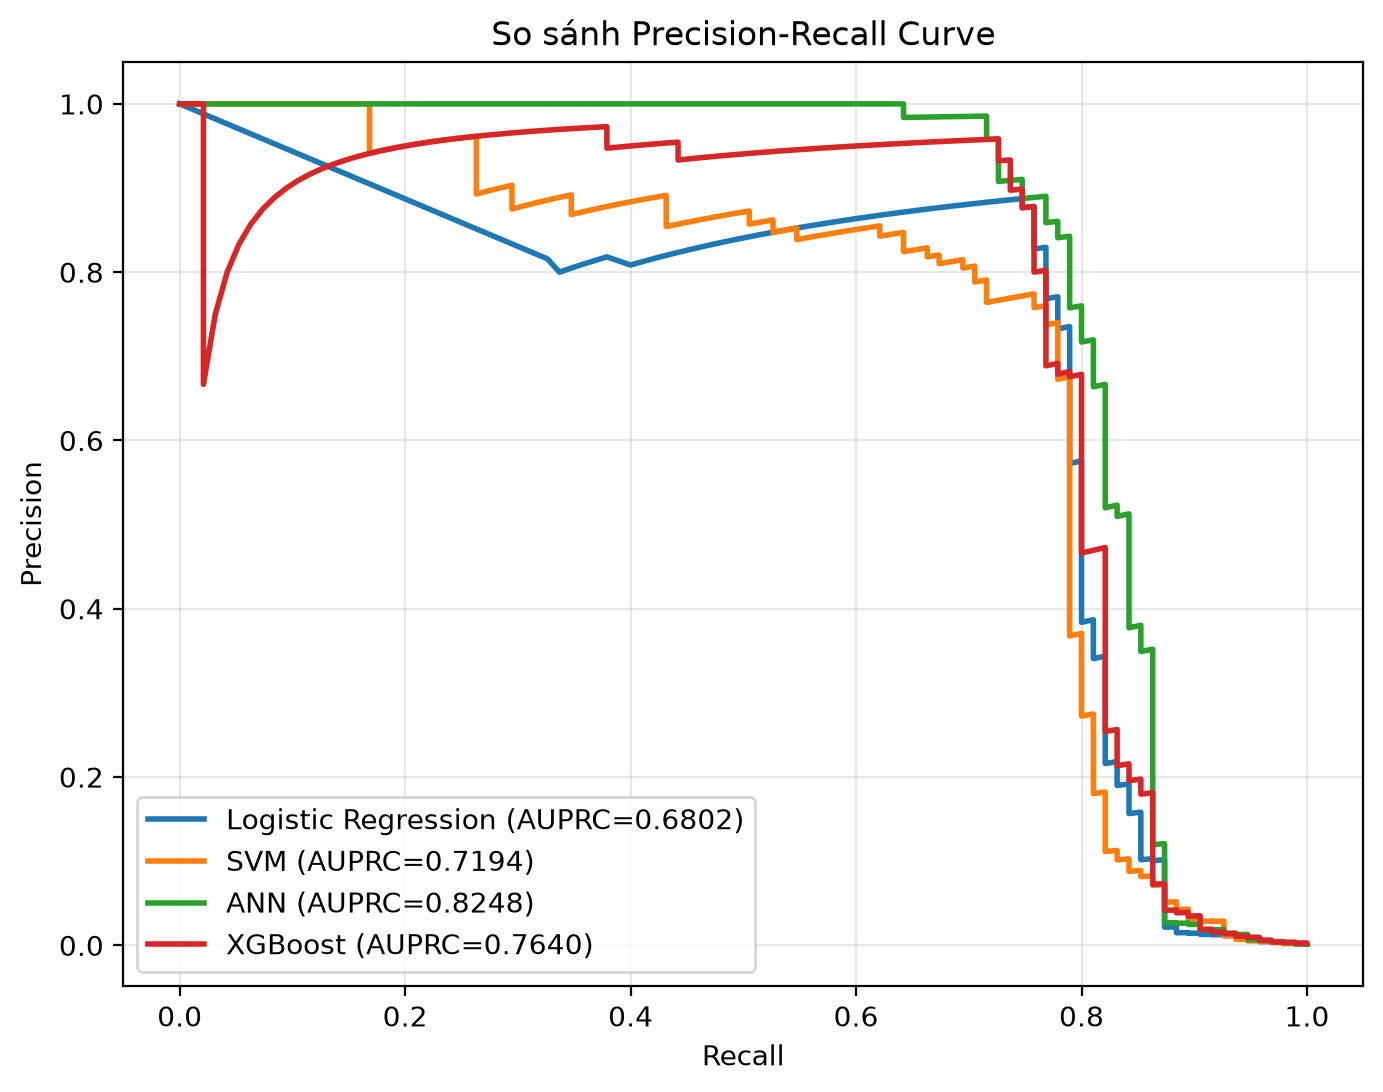
\includegraphics[width=0.8\linewidth]{graphics/compare_pr_curves.png}
\caption{So sánh đường cong Precision--Recall của các mô hình.}
\label{fig:so-sanh-pr}
\end{figure}

Hình~\ref{fig:so-sanh-metric} so sánh bốn metric chính giữa các mô hình. Có thể thấy Logistic Regression nổi bật ở Recall nhưng rất thấp ở Precision và F1, trong khi ANN và XGBoost cân bằng hơn giữa các metric.

\begin{figure}[H]
\centering
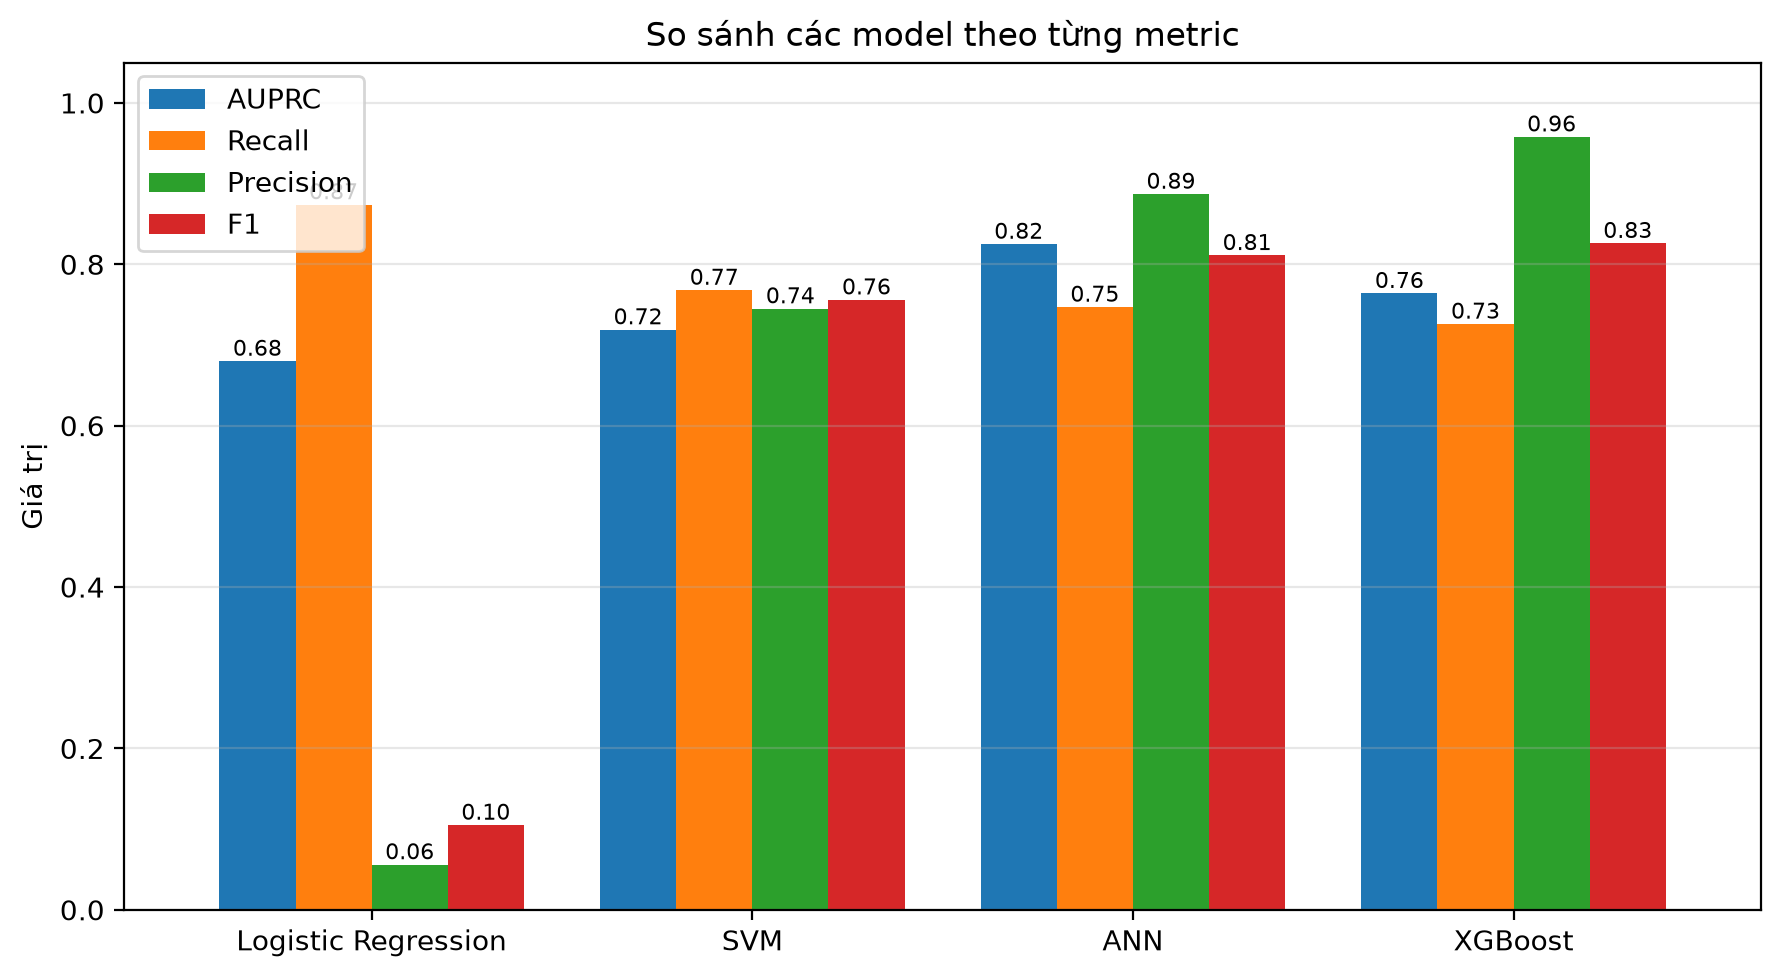
\includegraphics[width=0.85\linewidth]{graphics/compare_metrics_bar.png}
\caption{So sánh AUPRC, Recall, Precision và F1 của các mô hình.}
\label{fig:so-sanh-metric}
\end{figure}

Hình~\ref{fig:so-sanh-cm} thể hiện ma trận nhầm lẫn của từng mô hình tại $\tau = 0{,}5$ (hàng là nhãn dự đoán, cột là nhãn thực). Hình~\ref{fig:so-sanh-loi} cho thấy số lượng hai loại lỗi: $FN$ (bỏ sót gian lận) và $FP$ (báo nhầm giao dịch hợp lệ). Logistic Regression có ít $FN$ nhất ($12$) nhưng nhiều $FP$ nhất ($1\,403$), còn XGBoost có ít $FP$ nhất ($3$) nhưng nhiều $FN$ nhất ($26$).

\begin{figure}[H]
\centering
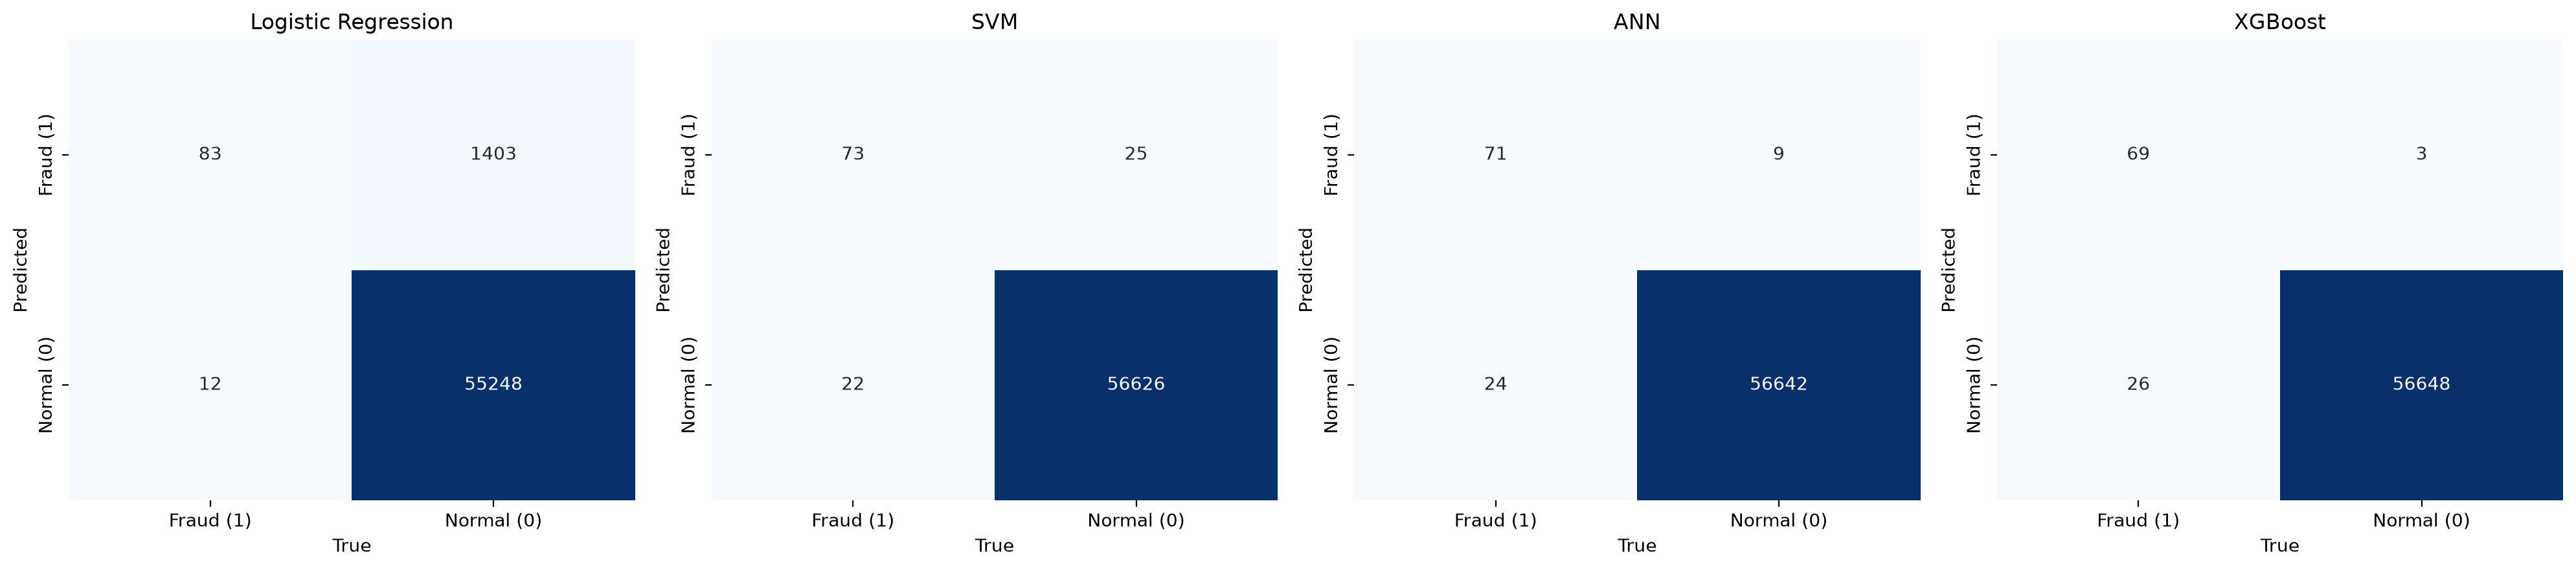
\includegraphics[width=\linewidth]{graphics/compare_confusion_matrices.png}
\caption{Ma trận nhầm lẫn của các mô hình trên tập kiểm tra ($\tau = 0{,}5$).}
\label{fig:so-sanh-cm}
\end{figure}

\begin{figure}[H]
\centering
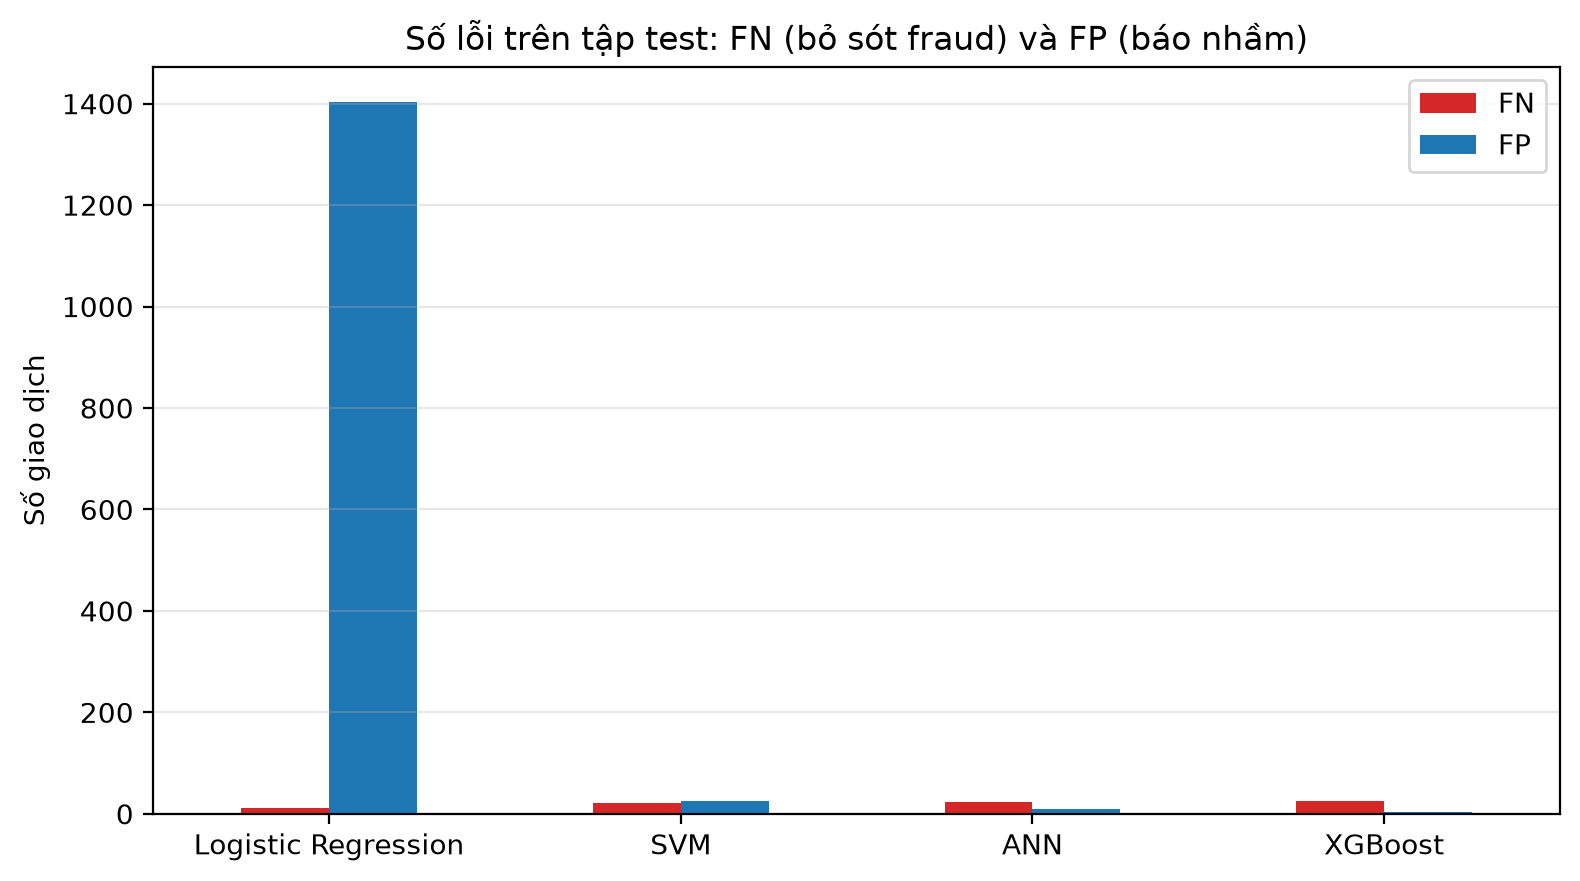
\includegraphics[width=0.75\linewidth]{graphics/compare_errors.png}
\caption{Số lượng $FN$ và $FP$ của các mô hình trên tập kiểm tra.}
\label{fig:so-sanh-loi}
\end{figure}

Cuối cùng, Hình~\ref{fig:threshold-sweep} thể hiện sự thay đổi của Precision, Recall và F1 theo ngưỡng $\tau$ cho từng mô hình. Với ANN và XGBoost, F1 duy trì ở mức khoảng $0{,}81$--$0{,}83$ trên một dải ngưỡng rộng (xấp xỉ $0{,}2$ đến $0{,}8$), nên ngưỡng mặc định $\tau = 0{,}5$ nằm trong vùng gần tối ưu và kết quả ít nhạy với ngưỡng. SVM cũng cho F1 ổn định ở mức $0{,}73$--$0{,}76$ khi $\tau \gtrsim 0{,}4$, nhưng F1 giảm mạnh khi $\tau$ nhỏ hơn khoảng $0{,}35$. Logistic Regression khác biệt rõ rệt: do dùng \texttt{class\_weight=balanced}, xác suất đầu ra bị đẩy cao nên Precision thấp hơn $0{,}2$ với mọi $\tau$ dưới khoảng $0{,}8$, và F1 chỉ tăng khi $\tau$ tiến gần $1$ (xấp xỉ $0{,}7$ tại $\tau \approx 0{,}99$). Như vậy, ngưỡng $0{,}5$ rất xa ngưỡng tối ưu của mô hình này, và F1 thấp ($0{,}105$) ở Bảng~\ref{tab:ket-qua-test} phần lớn là do ngưỡng chứ không hẳn do khả năng xếp hạng kém. Cần lưu ý rằng Hình~\ref{fig:threshold-sweep} được vẽ trên tập kiểm tra chỉ nhằm mục đích phân tích độ nhạy của các metric theo ngưỡng, các kết quả chính trong Bảng~\ref{tab:ket-qua-test} đều dùng ngưỡng cố định $\tau = 0{,}5$, không được điều chỉnh trên tập kiểm tra. Trong ứng dụng thực tế, ngưỡng cần được chọn trên tập validation hoặc bằng kiểm định chéo để tránh rò rỉ thông tin từ tập kiểm tra.

\begin{figure}[H]
\centering
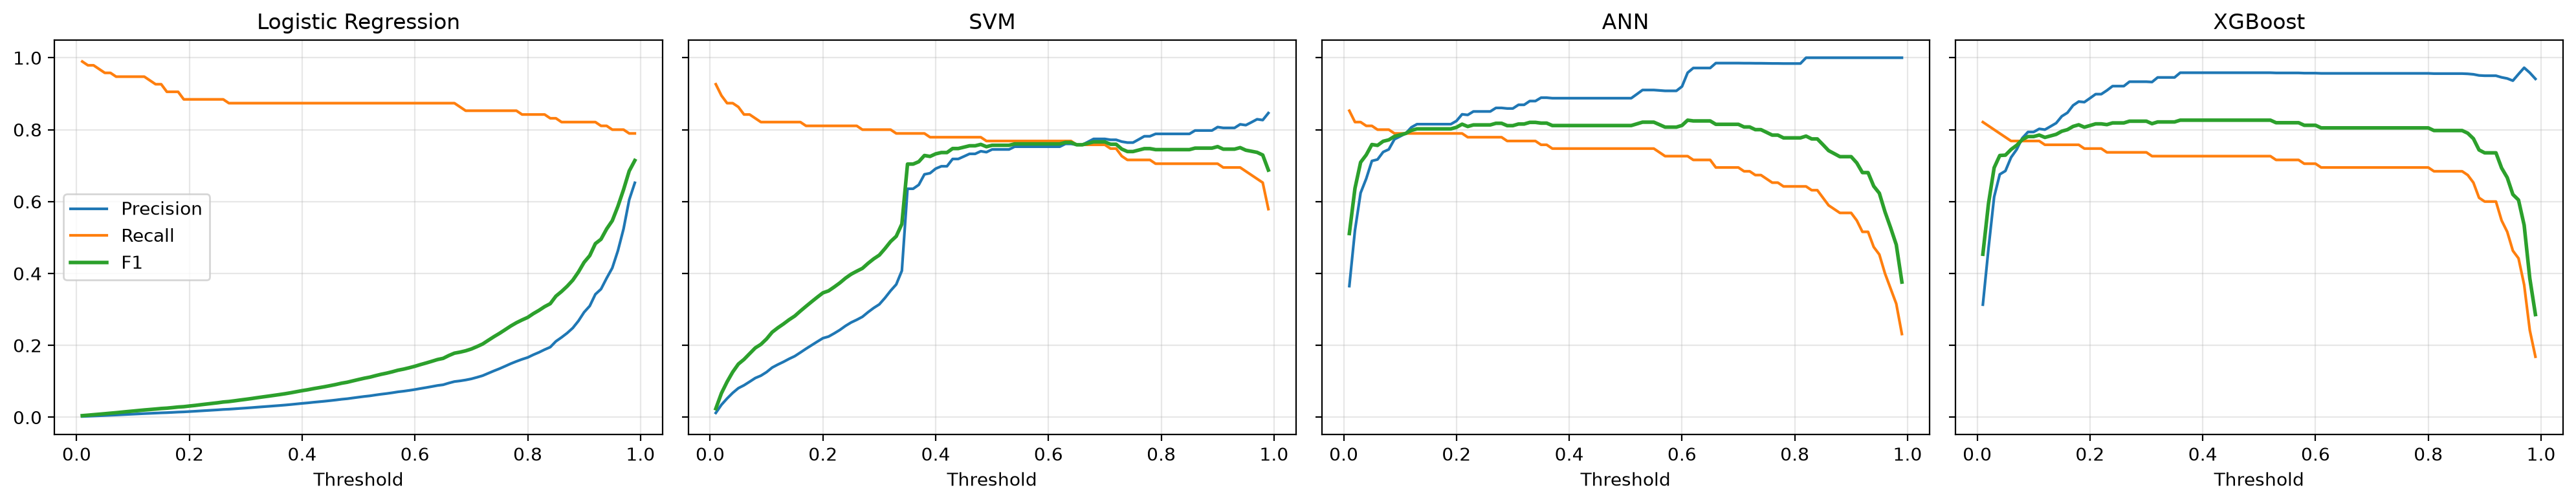
\includegraphics[width=\linewidth]{graphics/compare_threshold_sweep.png}
\caption{Precision, Recall và F1 theo ngưỡng quyết định $\tau$.}
\label{fig:threshold-sweep}
\end{figure}
